\kapitola{Úvod a cíl práce}
\sekce{Úvod do problematiky}
S růstem výpočetního výkonu a rozvojem \textbf{gpugpu} (paralelizace výpočtů na grafické kartě) se neuronové sítě ukázaly jako mocný nástroj pro řešení složitých problémů na které standardní metody umělé inteligence nestačily. Především díky jejích schopn


\kapitola{Neuronové sítě}

Neuronové sítě jsou model strojového učení, který je volně založený na principu zvířecího mozku. \cite[s.~41]{fundementalsOfDeepLearning}
\sekce{Neuron}
Neuron je základní jednotka neuronových sítí, která je definovaná jako suma všech jejích vstupů a aplikace aktivační funkce.
	$$\sigma(\Sigma_{i=0}^{N} \theta \cdot x_{i} + b)$$

\podsekce{Aktivační funkce}
Aktivační funkce se používá pro definování výstupu a zavedení nelinearity. Bez nich by byla neuronová síť schopna aproximovat pouze n-dimenzionální rovinu. Dalším využitím   \cite[s.~65]{fundementalsOfDeepLearning}

\podsekce{Linearní funkce}
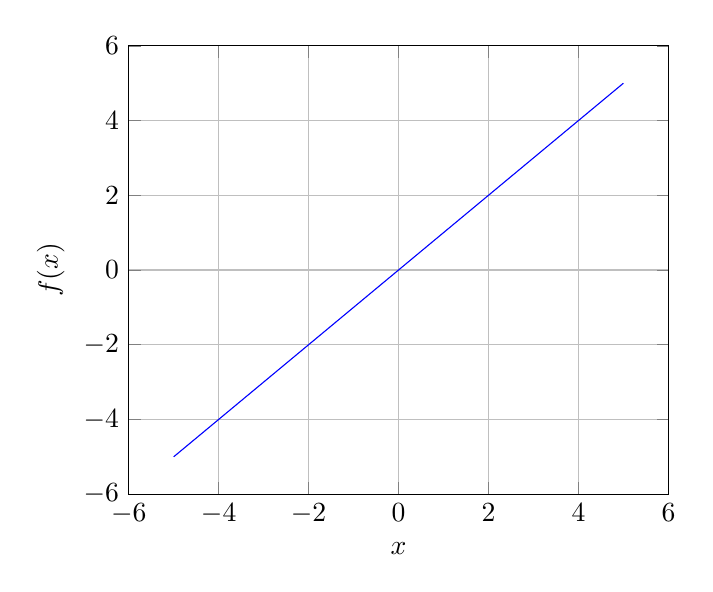
\begin{tikzpicture}
\begin{axis}[grid=major, xlabel=$x$, ylabel={$f(x)$}]
\addplot[blue, samples=100, smooth, unbounded coords=discard]
plot (\x, \x);
\end{axis}
\end{tikzpicture}
$$f(x) = x$$
\podsekce{Sigmoid}
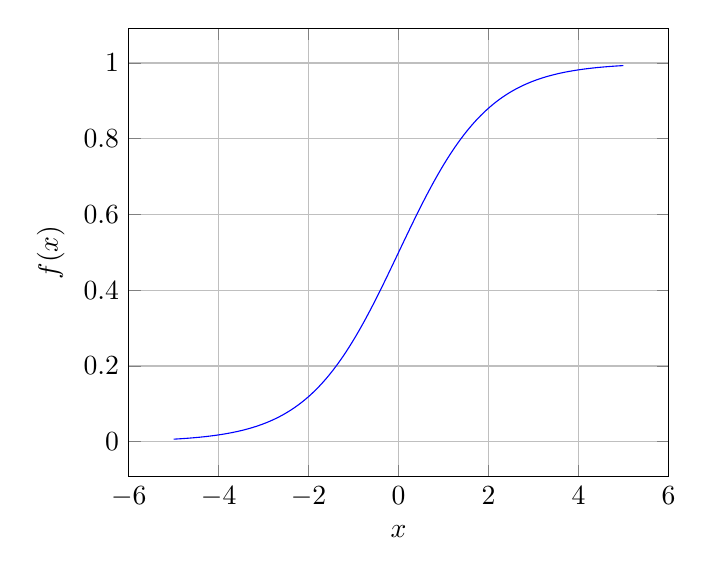
\begin{tikzpicture}
\begin{axis}[grid=major, xlabel=$x$, ylabel={$f(x)$}]
\addplot[blue, samples=100, smooth, unbounded coords=discard]{1 / (1 + e ^ (-\x))};
\end{axis}
\end{tikzpicture}
$$f(x) = \frac{1}{1 + e^{-x}}$$
\podsekce{Tanh}
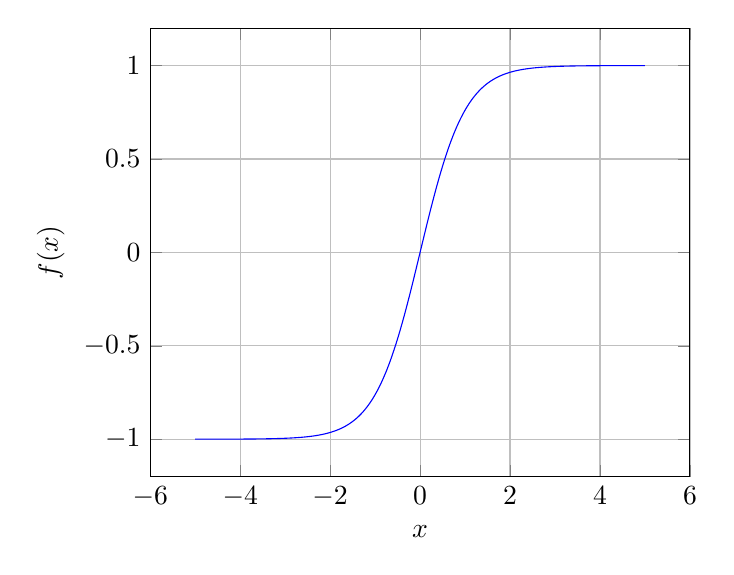
\begin{tikzpicture}
\begin{axis}[grid=major, xlabel=$x$, ylabel={$f(x)$}]
\addplot[blue, samples=100, smooth, unbounded coords=discard]{tanh(x)};
\end{axis}
\end{tikzpicture}
$$f(x) = tanh(x)$$
\podsekce{RELU}
RELU je aktivační funkce, která je podobná lineární aktivační funkci s tím rozdílem, že pokud vstupní hodnota nepřesáhne určitého prahu výstupem je 0. \cite[s.~69]{fundementalsOfDeepLearning} \\
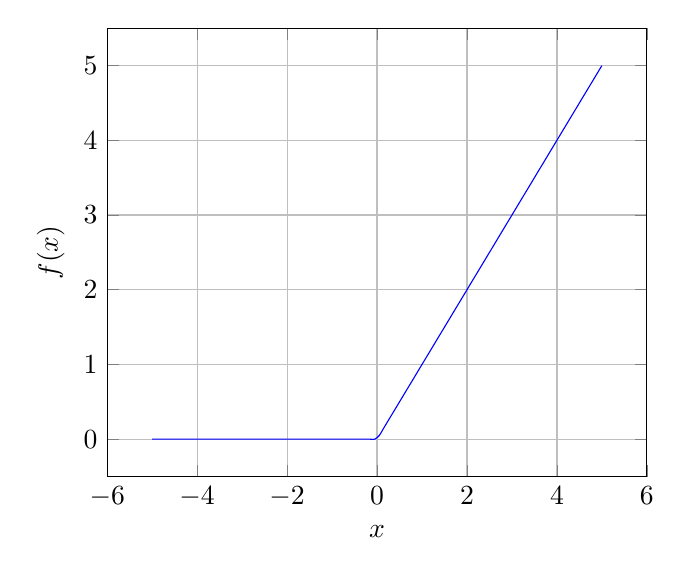
\begin{tikzpicture}
\begin{axis}[grid=major, xlabel=$x$, ylabel={$f(x)$}]
\addplot[blue, samples=100, smooth, unbounded coords=discard]{max(0, x)};
\end{axis}
\end{tikzpicture}
\[ 
f(x) = 
\begin{dcases*} 
\text{$x>=0$,} & $x$ \\ 
\text{$x<0$,} & 0 
\end{dcases*} 
\]